\documentclass[aspectratio=169]{beamer}
\setbeamertemplate{navigation symbols}{}
\usepackage{color,amsmath,comment, subfigure}
\usepackage{booktabs}
\usepackage{url}

\def\imagetop#1{\vtop{\null\hbox{#1}}} %http://tex.stackexchange.com/questions/23521/tabular-vertical-alignment-to-top

%%%%%%%%%%%%%%%%%%%%%%%%%%
\title[]{Lecture 23: Who knows what about who?}
\author[]{Matthew J. Salganik}
\institute[]{Sociology 204: Social Networks\\Princeton University}
\date[]{
Pre-read
\vfill

\begin{flushleft}
\vspace{0.6in}

\includegraphics[width=0.1\textwidth]{figures/cc.png}
\end{flushleft}
}

\note{
More compare and contrast of three studies:
- design (interview of alters vs guess what alter will say, game of contacts doesn't ask actual alter info)
- goals (basic vs applied)
}

\begin{document}
%%%%%%%%%%%%%%%%%%%%%%%%%%%
\frame{\titlepage}
%%%%%%%%%%%%%%%%%%%%%%%%%%%
\begin{frame}

\begin{center}
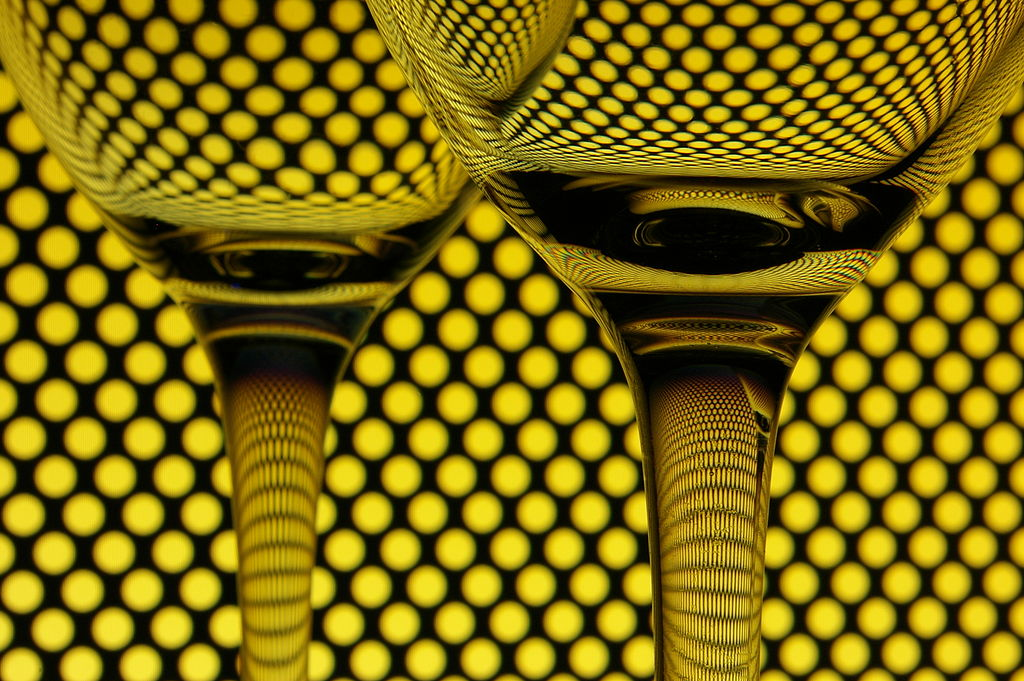
\includegraphics[width=0.8\textwidth]{figures/distortion.jpg}
\end{center}

\vfill
\tiny{\url{https://commons.wikimedia.org/wiki/File:Uniformity.jpg}}

\note{
What you see is distorted
}

\end{frame}
%%%%%%%%%%%%%%%%%%%%%%%%%%%
\begin{frame}

\begin{itemize}
\item your perception of the social world is distorted
\pause
\item your perception of your own social world is distorted
\end{itemize}

\pause 
Why do we care?

\begin{itemize}
\item interesting \pause
\item impacts social influence \pause
\item potentially creates social stasis \pause
\item important for scale-up method
\end{itemize}

\end{frame}
%%%%%%%%%%%%%%%%%%%%%%%
\begin{frame}

\begin{itemize}
\item Salganik et al. (2011) Motivated by the scale-up method 
\item Cowen (2014) Motivated by social visibility and attitude change more generally
\end{itemize}

\end{frame}
%%%%%%%%%%%%%%%%%%%%%
\begin{frame}

Enjoy the readings 

\end{frame}

\end{document}
